\documentclass[conference]{IEEEtran}
\IEEEoverridecommandlockouts
\usepackage{cite}
\usepackage{amsmath,amssymb,amsfonts}
\usepackage{algorithmic}
\usepackage{graphicx}
\usepackage{textcomp}
\usepackage{xcolor}
\usepackage{lipsum}
\usepackage{blindtext}
\usepackage{subfig}
\usepackage{caption}
\usepackage{placeins}
\usepackage{afterpage}
\usepackage{xurl}
\usepackage{gensymb}
\usepackage{stmaryrd}
\graphicspath{{./images/}}

\definecolor{light-gray}{gray}{0.95}
\newcommand{\size}[2]{{\fontsize{#1}{0}\selectfont#2}}
\newcommand{\code}[1]{\colorbox{light-gray}{\size{8}{\texttt{#1}}}}
\newcommand{\monospace}[1]{\size{8}{\texttt{#1}}}

\def\BibTeX{{\rm B\kern-.05em{\sc i\kern-.025em b}\kern-.08em
    T\kern-.1667em\lower.7ex\hbox{E}\kern-.125emX}}

\begin{document}

\title{Model-Free Deep Reinforcement Learning Algorithms in the MuJoCo Physics Simulator}

\author{
    \IEEEauthorblockN{Curtis Brinker}
    \IEEEauthorblockA{cjbzfd@mst.edu}
    \and
    \IEEEauthorblockN{Tanner May}
    \IEEEauthorblockA{tmay@mst.edu}
}
\maketitle

\begin{abstract}
    Deep reinforcement learning is a field that has show rapid growth in the recent years. These advances have made progress in solving problems that were previously considered unapproachable such as the game Go or self driving vehicles. This paper looks to provide an introduction to deep reinforcement learning by examining several notable algorithms in detail. These algorithms are then implemented and tested in the MuJoCo physics simulation to provide quantitative and qualitative comparisons of the performance for each of the different algorithms.
\end{abstract}

\section{Introduction}

Recent developments in machine learning have made huge strides in approaching problems that were previously unsolvable with traditional programming methods. In general, machine learning techniques are grouped into three categories: supervised learning, unsupervised learning, and reinforcement learning (RL). The first two categories train on a dataset with constant values. RL is unique in the fact that the data it trains on frequently changes due to the strong causal interdependency between the agent and the environment. As the training data is consistently changing, RL algorithms must be able to learn in real time, called online learning \cite{rl_application}.

This paradigm of machine learning aligns well with several real life applications and as a result has led to new state-of-the-art algorithms to solve them.  Some examples may include DeepMind's AlphaZero, which became the best Go player. Another example are RL algorithms that have achieved superhuman performance in a variety of Atari games using only visual inputs. However, RL algorithms can excel in more than just games, RL agents have been created to control robotics, design machine learning algorithms and much more \cite{deep_rl_survey}.

RL is capable of learning on data as it comes in. This data is formulated as a set of interactions with the agent's environment where each interaction consists of the state of the environment,the action the agent performed, and the resulting state. Thus, agents that use RL learn with a circular process that is a result of the agent's previous actions, known as the agent-environment interaction loop. This complex relationship has given rise to multitudes of algorithms, from remembering a mapping between states and actions to using multiple neural networks to determine the next action .

In this paper we aim to give an introduction to the mathematics used in deep reinforcement learning by examining several famous deep RL algorithms. By learning the mathematics, we aim to learn the core principles that the field of RL uses, along with special tricks and techniques that are used to improve performance. Specifically, this paper looks to study and implement the following algorithms:
\begin{itemize}
    \item REINFORCE
    \item A2C
    \item DDPG
    \item SAC
\end{itemize}

To test the performance of these algorithms, we trained models and recorded the improvement over time. The most intensive tests were performed in the MuJoCo simulator where agents were trained to walk in a 3D simulation. All code, models and figures from these tests are available at the project repo.\footnote{\label{repo}https://github.com/cubrink/mujoco-2.1-rl-project}

\section{Testing Environment}

All algorithms were written and tested on a Linux system running Ubuntu 20.04. The system had the MuJoCo 2.1 installed according to the instructions provided in the project repo.\footnotemark[\ref{repo}] MuJoCo stands for {\bf Mu}lti-{\bf Jo}int dynamics with {\bf Co}ntact and was made for applications that require fast, accurate physics simulations such as robotics and machine learning \cite{mujoco_docs}. Using MuJoCo, machine learning algorithms can learn how to control the movement of robotic models, such as a snake, ant, or humanoid.

All RL algorithms were written using Python 3.8 and the PyTorch library. The algorithms were written using the OpenAI \code{gym} interface. This interface was used as it is a standardized way to interact with RL algorithms and the \code{gym} library has native support for MuJoCo. This interface is described in the documentation \cite{gym_docs}. An overview of this interface is given below:

\begin{itemize}
    \item \code{reset()}: Resets the environment to an initial state
    \item \code{step()}: Used to update the environment and returns the following:
          \begin{itemize}
              \item An observation of the environment
              \item The reward from the most recent step
              \item A done flag, marking a state as a terminal state
              \item An info object which has a log of the internal details of the environment step
          \end{itemize}
\end{itemize}

\section{Background}

The study of reinforcement learning is about training an \textit{agent} to interact with an \textit{environment}. An action by an agent can influence the environment, which may later affect the actions of the agent. For this reason, reinforcement learning algorithms must be able handle a changing environment that is causally influenced by the agent itself.

Formalizing the interdependency between the environment and the agent is done with the \textit{agent-environment interaction loop}. In which, at time $t$ the environment is fully described by its \textit{state}, $s_t$. Then, an agent makes an \textit{observation} of the environment, $o_t$, where $o_t \subseteq s_t$.\footnote{While the observation and the state are not necessarily equal, reinforcement learning literature frequently refers to an observation as the state itself.} The agent responds to this observation with an \textit{action} $a_t$ and is given a \textit{reward}, $r_t$. After the action is taken, the state of the environment changes with the new state denoted as $s_{t+1}$.

An environment state can be represented by a tensor of values describing individual aspects of the environment. The domain of possible observations of the agent is referred to as the \textit{observation space}, which can be either continuous or discrete. Similarly, the domain of all actions that an agent can take is called the \textit{action space} which can also be continuous or discrete. An action, $a_t$, is selected from the action space by agent's \textit{policy}. The policy can select actions either deterministically or stochastically. Typically, deterministic policies are denoted with $a_t = \mu(s_t)$ and stochastic policies are denoted as $a_t \sim \pi(\cdot | s_t)$ \cite{spinning_up_intro}.



The reward given for the transition from $s_t$ to $s_{t+1}$ by action $a_t$ is given by the reward function, where $r_t = R(s_t, a_t, s_{t+1})$. Though, readers should be aware that some literature refers to this value as $r_{t+1}$. Typically, this reward function is specified by a programmer in a way that rewards a specific goal. With this in mind, the process of training an agent can be formulated as maximizing the cumulative reward, called the \textit{return}. To calculate the return, the \textit{trajectory} is used which contains the sequence of states and actions taken by the agent. The trajectory is given by:
$$
    \tau = (s_0, a_0, s_1, a_1, ...)
$$

Therefore, as the return is defined in terms of cumulative reward, the trajectory can be used to calculate the rewards as the agent interacts with the environment. Then, in its most simple form, the return is the summation of all rewards. However this introduces two problems: First the return for an action $t$ is defined in terms of actions taken before it. Intuitively, we would to only consider rewards that will happen as a result of the current action. Second, The summation of all rewards weights all rewards equally, however, this means that very long term rewards may eventually dominate the summation. To encourage shorter term rewards we can introduce a discount factor, $\gamma$, that discounts the value of future rewards.

Commonly, the reward function $R$ is co-opted to take a trajectory and produce the rewards at each timestep $t$. With these considerations in mind, the return can be defined as:
$$
    R_t(\tau) = \sum_{t'=t}^T \gamma^{t'} r_{t'}, \enspace \gamma \in (0, 1)
$$

Where $T$ is the length of the trajectory and $t$ is the current time for which the return is being calculated. If $T$ is finite, then the return is said to be a \textit{finite-horizon return}. Similarly, if $T$ is infinite, then the return is said to an \textit{infinite-horizon return}. The inclusion of $\gamma$ makes this return a discounted return. This places more focus on near-term rewards and also helps with convergence in infinite-horizon returns. Using $t'$ makes the return only consider future rewards, which \cite{spinning_up_policy_optimization} calls the \textit{reward-to-go} return.

However, an agent cannot act to directly maximize its return as it dependent on future actions and states. Instead, an approximation must be used to calculate the expected return, $\mathcal{J}(\pi)$. This this done with \textit{value functions}. Formally, $\mathcal{J}(\pi)$ is defined as:
$$
    \mathcal{J}(\pi) = \mathop{\mathbb{E}}_{\tau \sim \pi}[R(\tau)]
$$

The \textit{state value function} for policy $\pi$, denoted as $V^\pi$, gives the expected value for policy $\pi$ given state $s$. Alternatively, the \textit{state-action value function} for policy $\pi$, denoted as $Q^\pi$, which can be used estimate the expected value for policy $\pi$ in state $s$ and immediately taking action $a$. Formally, these are defined as:
\begin{align*}
    V^\pi(s)    & = \mathop{\mathbb{E}}_{\tau \sim \pi}[R(\tau) \, | \, s_0 = s]          \\
    Q^\pi(s, a) & = \mathop{\mathbb{E}}_{\tau \sim \pi}[R(\tau) \, | \, s_0 = s, a_0 = a]
\end{align*}

However, these functions are still dependent on the return. To avoid this, we can use the Bellman Equations, which defines both $V^\pi$ and $Q^\pi$ in terms of expected values of future states. \cite{deep_rl_survey, spinning_up_intro, sutton2018reinforcement} These equations are given as:
\begin{align*}
    V^\pi(s)    & = \mathop{\mathop{\mathbb{E}}_{a \sim \pi}}_{s' \sim P} \left[ R(s, a, s') + \gamma V^\pi(s')\right]                  \\
    Q^\pi(s, a) & = \mathop{\mathbb{E}}_{s' \sim P} \left[ R(s, a, s') + \gamma\mathop{\mathbb{E}}_{a' \sim \pi} [Q^\pi(s', a')]\right] \\
                & = \mathop{\mathbb{E}}_{s' \sim P}\left [ R(s, a, s') + \gamma V^\pi(s') \right]
\end{align*}
\begin{flushleft}
    Where $P$ is the environment state transition function and $s'$ is the resulting state.
\end{flushleft}


For the agent to maximize $\mathcal{J}(\pi_\theta)$, the agent must learn to improve the policy $\pi_\theta$, where $\theta$ are the parameters for the policy and is normally updated by gradient ascent. Normally this involves using $V^\pi$ or $Q^\pi$ to better approximate the optimal value functions. Commonly, these approximation are done via deep neural networks. The exact details of how the policy and value function(s) are updated is dependent on the reinforcement learning algorithm used. Following is a brief discussion on different types of reinforcement learning algorithms followed by discussions on details of specific algorithms studied in this paper.

A simplified taxonomy of deep reinforcement learning algorithms is given by \cite{spinning_up_taxonomy}. At the highest level, reinforcement learning algorithms can be split into two categories, \textit{model-based} or \textit{model-free}. Model-based algorithms learn the state transition function, allowing it to predict future states of the environment. Learning the world model has many benefits that can drastically increase the performance of an agent, however, doing so significantly increases the complexity of the algorithms and is outside the scope of this paper. Model-free algorithms do not learn to predict the environment and instead learn other functions to increase the agent's return. Model-free algorithms can be further categorized as using \textit{policy optimization} or \textit{Q-learning}.\footnote{Policy optimization and Q-learning are not mutually exclusive categories.}

Policy optimization algorithms train by optimizing the parameters of the policy $\pi_\theta$. This is normally done learning a value approximator $V_\phi$ and sampling actions taken by the current policy to update parameters accordingly. Because this process requires actions from the current policy, these techniques are considered to be \textit{on-policy}.

Another approach, though not necessarily mutually exclusive, is using Q learning. These algorithms learn an approximator $Q_\theta$ to determine the value of state action pairs. An advantage to this technique is that it can learn from past experiences that were not from the current policy. Algorithms that can learn from experiences of different policies are called \textit{off-policy}. Actions by these algorithms typically are chosen by selecting the action that maximizes $Q_\theta(s, a)$ for the current state $s$.

\subsection{The REINFORCE Algorithm}

One of the simplest forms of policy optimization algorithms is a class of algorithms presented by Williams as REINFORCE \cite{REINFORCE}. The core idea this algorithm is to update the policy by sampling trajectories from the policy. Once a sample has been taken from the current policy, the policy $\pi_\theta$ and value approximator $V_\phi$ can be updated. There is some flexibility in how the parameters are updated, though \cite{spinning_up_policy_optimization} provides some examples of frequently used techniques. The policy is updated using gradient ascent where the gradient is given by:
$$
    \nabla_\theta\mathcal{J(\pi_\theta)} = \mathop{\mathbb{E}}_{\tau \sim \pi_\theta} \left[\sum_{t=0}^{T}\nabla_\theta \, log \, \pi_\theta(a_t | s_t) \, \Phi_t \right]
$$
\begin{flushleft}
    Where $\Phi_t$ is any function that is independent of $\theta$.
\end{flushleft}


To update the value approximator parameters $\phi$, it is common to use gradient descent on a loss such as mean squared error on the value approximator and the reward-to-go return.
$$
    \mathcal{L}(\phi) = \mathop{\mathbb{E}}_{\tau \sim \pi_\theta} \left[\left(V_\phi(s_t) - R_t(\tau)\right)^2\right]
$$

\subsection{Advantage Actor Critic (A2C)}

The advantage actor critic is an on-policy algorithm based on the REINFORCE algorithm. A2C was first proposed by \cite{A2C} along with an asynchronous variant called A3C. The details about the asynchronous version of the algorithm is not pertinent to this paper and will not be discussed. As a whole, there are two main techniques used to improve the performance of this algorithm.

The first technique is the use of the advantage function, $A^{\pi_\theta}(s_t, a_t)$ as $\Phi_t$. The advantage function is defined as:
$$
    A^{\pi_\theta}(s_t, a_t) = Q^{\pi_\theta}(s_t, a_t) - V^{\pi_\theta}(s_t, a_t)
$$

It should be noted that $\Phi_t$ must be independent of $\theta$ and by consequence $a_t$. However, \cite{spinning_up_policy_optimization} provides a proof that $A^{\pi_\theta}(s_t, a_t)$ can be written it terms of $s_t$ only. The advantage can be thought of as quantifying how much better an action in a given state is than average. Negative values signify that the action was less than the expected value for the given state, and positive signifies that it was better. Mathematically, the advantage function is useful as subtracting by $V^{\pi_\theta}(s_t)$ reduces the variance in the policy gradient leading to more stable learning.

The second technique is the use of an actor-critic framework. The idea of this framework it to separate the concerns of learning different aspects of training. The actor is tasked with learning the policy that will interact with the environment. The critic is tasked with learning the value function that it will use to criticize the actor's actions \cite{deepmind_slides_9}.

\subsection{Deep Deterministic Policy Gradient (DDPG)}

DDPG is an off-policy learning algorithm for continuous action spaces that was proposed by \cite{DDPG}. It learns a Q function and a deterministic policy to select actions and uses a variety of techniques to improve performance and stability of the algorithm. An overview of unique methods used by this algorithm is provided by \cite{spinning_up_ddpg}. One technique that is commonly used by off-policy algorithms is the use a replay buffer. Because off-policy algorithms can learn from actions that did not originate from the current policy, past experiences can be stored in a buffer. Then, during training, a larger sample size can be used to improve training.

To update the function $Q_\phi$, gradient descent is used on $\phi$ to minimize the mean squared error of $Q_\phi(s, a)$ and the \textit{target}, where the target is defined as:
$$
    y = r + \gamma(1-d)Q_\phi(s', \mu_\theta(s'))
$$

Where $(s, a, r, s', d)$ is a transition in the replay buffer $\mathcal{D}$. The resulting state from the action is $s'$ and $d$ is the \textit{done} flag where $d=1$ if $s'$ is a terminal state, $d=0$ otherwise. Additionally, $\mu_\theta$ is the deterministic policy used to select the next action.

However, using gradient descent on the mean squared error of $Q_\phi$ and $y$ is problematic as $y$ is also dependent on $\phi$. As a result, both $Q_\phi$ and $y$ change when $\phi$ is updated, leading to instability. To resolve this, DDPG uses \textit{target networks}, which uses polyak averaging to remove this direct dependency. The target networks, $Q_{\phi'}$ and $\mu_{\theta'}$ have the same structure as their original networks but are updated as follows:
\begin{align*}
    \phi'   & \leftarrow \tau \, \phi' + (1 - \tau) \phi     \\
    \theta' & \leftarrow \tau \, \theta' + (1 - \tau) \theta
\end{align*}

\begin{flushleft}
    For $\tau \in (0, 1)$. This provides stability to the loss function, therefore $Q_\phi$ is updated using gradient descent on
\end{flushleft}

$$
    \mathcal{L}(\phi, \mathcal{D}) = \mathop{\mathbb{E}}_{(s,a,r,s',d) \sim \mathcal{D}}\left[\left(Q_\phi(s,a) - y\right)^2\right]
$$
This loss function is called the Mean Square Bellmen Error (MSBE) where $y$ is the target, which is calculated as:
$$
    y = r + \gamma(1-d)Q_{\phi'}(s', \mu_{\theta'}(s'))
$$

To update the policy, we want to maximize the value function $Q_\phi$ using $\mu_\theta$. To do this, the following loss function is used:
$$
    \mathcal{L}(\theta, \mathcal{D}) = \mathop{\mathbb{E}}_{s \sim \mathcal{D}}\left[-Q_\phi(s, \mu_\theta(s))\right]
$$

Finally, to gain additional benefit from the algorithm off-policy, DDPG uses another technique to encourage exploration during train time. This is done by adding random noise to actions to stray away from the deterministic policy. The original authors uses OU noise, however \cite{spinning_up_ddpg} recommends a zero centered Gaussian distribution which is simpler to implement and still effective.

\subsection{Soft Actor Critic (SAC)}

The Soft Actor Critic Algorithm is an stochastic off-policy algorithm that uses an actor-critic framework and entropy regularization. This algorithm was originally proposed by \cite{SAC1, SAC2}, additionally, a guided explanation is given by \cite{spinning_up_sac}. SAC can be implemented for either discrete or continuous action spaces, however, the details that follow will be tailored for the continuous version.

SAC works by learning a stochastic policy $\pi_\theta$ and two $Q$ functions, $Q_{\phi_1}$ and $Q_{\phi_2}$.  When evaluating the value, the minimum value is taken between $Q_{\phi_1}(s, a)$ and $Q_{\phi_2}(s, a)$. This is called the \textit{clipped double-Q method}. Using this method helps prevent overestimating the value of state action pairs which improves training results.

Similar to DDPG, SAC uses target networks to stabilize the updates using the loss function. Unlike DDPG, SAC only uses target networks for value functions, not for policy. The parameters for the target networks are updated using polyak averaging as shown below:
\begin{align*}
    \phi_1' & \leftarrow \tau \, \phi_1' + (1 - \tau) \phi_1 \\
    \phi_2' & \leftarrow \tau \, \phi_2' + (1 - \tau) \phi_2
\end{align*}

\begin{flushleft}
    For $\tau \in (0, 1)$.
\end{flushleft}

To control exploration of the policy, SAC uses entropy regularization, where entropy is defined as:
$$
    H(P) = \mathop{\mathbb{E}}_{x \sim P} \left[- log \, P(x)\right]
$$
\begin{flushleft}
    For any distribution $P$. Roughly speaking, entropy measures how random a distribution is. An entropy of zero is given by a policy where where an action has probability 1. Larger values of entropy indicate more evenly spread probability distribution. The choice of entropy regularization is controlled with the entropy hyperparameter, $\alpha$, where $\alpha \in (0, 1)$. The greater the value of $\alpha$, the more the policy will explore.
\end{flushleft}

Entropy is introduced in several aspects of the SAC algorithm. The first is in the \textit{entropy regularized double-Q clipped target}, which is calculated as:
$$
    y = r + \gamma(1-d)\left(\mathop{min}_{k=1,2}Q_{\phi'_k}(s', a') - \alpha \, log \, \pi_\theta(a' \, | \, s')\right)
$$

\begin{flushleft}
    Where $a' \sim \pi_\theta$.
\end{flushleft}

This is used to calculate the entropy regularized MSBE which is used as the loss function for $Q_{\phi_1}$ and $Q_{\phi_2}$, given by:
$$
    \mathcal{L}(\phi_k, \mathcal{D}) = \mathop{\mathbb{E}}_{(s,a,r,s',d) \sim \mathcal{D}}\left[\left(Q_{\phi_k}(s,a) - y\right)^2\right], \enspace k=1,2
$$
\begin{flushleft}
    Where $\mathcal{D}$ is the experience replay buffer.
\end{flushleft}

The policy $\pi_\theta$ is updated in a way similar to DDPG. The policy is updated by using gradient ascent to maximize the value function. Therefore the loss function for $\pi_\theta$ becomes:
$$
    \mathcal{L}(\theta, \mathcal{D}) = \mathop{\mathop{\mathbb{E}}_{s \sim \mathcal{D}}}_{a \sim \pi_\theta} \left[-\left(\mathop{min}_{k=1,2} Q_{\phi'_k}(s, a) - \alpha \, log \, \pi_\theta(a \, | \, s)\right)\right]
$$

There are two important details regarding sampling action $a$ from $\pi_\theta$ in the SAC algorithm. First, sampling is done from a normal distribution using the \textit{reparameterization method}. This makes the randomly sampled number differentiable, allowing for actions to backpropagate through the policy's parameters. The second detail is that the SAC policy squashes the action into a finite action space, with $tanh$. This is done as most action spaces have finite bounds while normal distributions have infinite support. By limiting the domain of the action to the action space, the policy is learned more efficiently.

\section{Methodology}

Testing of the effectiveness of RL algorithms was done sequentially and in multiple stages, increasing in difficulty. The first tests were algorithms that used a discrete action spaces, REINFORCE and A2C. The tests were performed in the \code{CartPole-v0} environment. These tests were qualitative in nature, with the goal seeing that the simplest algorithms were properly learning.

The second group of tests focused on testing the implementation of algorithms with a continuous action spaces, DDPG and SAC. The tests were performed in the \code{Pendulum-v1} environment. These tests were quantitative in nature and recorded the improvement of the agent over time.

The third group of tests focused on testing the performance of algorithms with a continuous action spaces. The algorithms tested were A2C, DDPG and SAC. The tests were performed in the MuJoCo \code{Ant-v3} environment. These tests were quantitative in nature and recorded the improvement of the agent over time.

The fourth test took the best performing algorithm from the third group of tests and subjected it to a more challenging environment, MuJoCo's \code{Humanoid-v3} environment. This environment has a larger observation and action space than the \code{Ant-v3} environment. This test was quantitative in nature and recorded the improvement of the agent over time.


The hyperparameters for each algorithm were as follows:
\begin{itemize}
    \item REINFORCE: Train for a maximum of 5000 episodes. Update at end of each episode. Learning rate of $3\text{e-}4$.
    \item A2C: Learning rate of $3\text{e-}4$ and $\gamma = 0.99$.
    \item DDPG: Update freq. of 64 steps, update threshold of 4096 steps, batch size of 128, learning rate of $1\text{e-}3$, $\gamma = 0.99$, $\tau = 0.995$, and the noise distribution was Gaussian with a standard deviation of 0.1.\footnote{\cite{DDPG} uses OU noise, but \cite{spinning_up_ddpg} recommends using Gaussian noise as it is easier to implement and gives similar results}
    \item SAC: Update freq. of 64 steps, 64 updates per update step, an update threshold of 4096 steps, batch size of 128, $\alpha = 0.5$, learning rate of $5\text{e-}4$, $\gamma = 0.99$, $\tau = 0.995$.
\end{itemize}
Each of those hyperparameters were chosen based roughly on existing literature. Values were tweaked until they resulted in a model that was capable of learning the environment.

All deep neural networks used in these algorithms were multilayer perceptrons with two hidden layers of size 256 each, using the ReLU activation function. From our testing, using 128 neurons per layer frequently caused problems when learning the environment. At 256 neurons, all models seemed to be able to learn the environment sufficiently and adding more neurons would have greatly increased the computational cost of training.

More detailed information about the tests in each environment is described in its own subsection below the source code for each environment is given by \cite {gym_source}.

\subsection{CartPole-v0}

The objective of the CartPole environment is to teach an agent to balance a pole on a cart by moving the cart left and right. The environment has a continuous observation space consisting of the cart's position, the cart's velocity, the pole's angle, and the pole's angular velocity. The action space is discrete with the options of moving the cart to the left or to the right. The environment rewards the agent with a value of one, simply for staying healthy.

When the environment is initialized the values of both the cart and pole are randomly sampled from a uniform distribution from $[-0.5, 0.5]$. The environment is terminated if: the angle of the pole is $\pm12\degree$ off center, the cart position hits the edge of the display,or when the length of the episode surpasses 200 steps. The environment is considered solved when the reward is\textgreater 195 for 100 consecutive episodes.

This environment was used as a qualitative test for the implementation of algorithms with a discrete action space.

\subsection{Pendulum-v1}

The pendulum environment's objective is to balance a frictionless pendulum straight up. The observation space is continuous and describes the angle of the pendulum as well as the angular velocity. The action space is also continuous and details the amount of left or right force to apply to the pendulum. The reward incentivizes keeping the pole at an angle of $0\degree$ with as little velocity and force as possible. The reward is formulated as
$$
    R = -(angle ^{2} + 0.1 * angular\_velocity ^ {2} + 0.001 * action ^ {2})
$$
Since the angle is normalized between $[-\pi, \pi]$ before calculating the reward, the reward has a range of$[-16.3, 0]$.

The environment's initial state has the pole at a random angle between $[-\pi, \pi]$ radians with a random velocity between $[-1, 1]$. The environment does not specify a termination state, so a limit of 150 steps was imposed. Similarly, the environment does not specify when it is solved, so it was allowed to run until it hit the step limit.

Similar to the CartPole environment, this environment was used to test the implementation of algorithms with continuous action spaces.

\subsection{Ant-v3}

The MuJoCo Ant-v3 environment has the goal of teaching an ant to move as quickly as possible to the right. The ant is a sphere with four legs, each with two joints. The continuous observation space is significantly more complex than the previous environments: it consists of the model's position, rotations, velocity, and the forces between the legs and the ground (contact force). The action space is also continuous and describes where and how quickly to move each joint. The reward encourages the model to move as quickly as possible while moving as few joints as little and softly as possible. It is formulated as
$$
    R = (v + h) - (a + f)
$$
where $v$ is the velocity in the x-axis, $h$ is the healthy reward configured to be 1, $a$ is the control\_cost calculated by $0.5* \sum actions^{2}$, and $f$ is the contact\_cost calculated by $5\text{e-}4 * \sum contact\_forces^{2}$.

The environment starts with each joint in a random position with a random velocity. The episode is terminated when the model exits the safe height range of $[0.3, 2.0]$. The environment did not define a solve condition so the episode was continued until the model made a mistake to trigger the termination condition.

The ant was chosen because it is the simplest provided model that meets the "three dimensional walker" condition. Each of the algorithms had 500,000 episodes to train using this model. After training was stopped, the most recently saved model was used for analysis. A training length of 500,000 episodes was used because it consistently produced an agent that could walk a non-trivial distance.

\subsection{Humanoid-v3}

The MuJoCo Humanoid-v3 environment has the goal of teaching an humanoid to move as quickly as possible to the right. The humanoid model is a humanoid with two legs, two arms, a head and a torso. The legs, arms, and torso are made up of multiple joints, each individually controlled. Like the ant, the observation space is continuous and describes the model's position, the model's velocity, the forces for each of the joints, and the contact forces. The environment also defines a continuous action space that describes the new position and velocity of each joint. The intuition for the reward is the same as for the Ant environment, but it is calculated slightly differently where $v$ is equal to $1.25 * x\_velocity$, $h$ is configured to be 5, $a$ is calculated as $0.1 * \sum actions^{2}$, and $f$ is defined as $5\text{e-}7 * \sum contact\_forces^{2}$.

Like the Ant environment, the model starts with each joint in a random position and random velocity. The episode is terminated when the model exits the safe height range of $[1.0, 2.0]$. The environment did not define a solve condition so the episode was continued until the model made a mistake to trigger the termination condition.

The humanoid was chosen because it is the most complex 3D walker and showcased the learning power of the tested algorithms. Since this model is significantly more complex than the Ant, 1,250,000 environment interactions were used for training. But due to the cost of training, only SAC was trained with this model.

\section{Results}

The following sections discuss each algorithms' results for each of the environments, including graphs of the reward history and various loss values. As \cite{spinning_up_intro} notes, unlike other machine learning techniques, supervised learning for example, the loss function is defined on the most recent policy, so it is only relevant for calculating the descent gradient \textit{for that specific version of the policy}. This means that minimizing the loss function is not guaranteed to improve the expected return, and may in fact do the opposite. Essentially, for RL the loss values mean nothing, but their graphs were included here for posterity's sake.

To see videos of the agents' performance in some of the following environments see \cite{agent_videos}.

\subsection{CartPole-v0}

The CartPole test was qualitative in nature and was used to provide feedback that the our earliest implementations of the algorithms were working. Both the REINFORCE and A2C algorithms were able to solve the environment in a matter of a few minutes. Qualitatively the A2C appeared to have better performance in this environment.

\subsection{Pendulum-v1}

\begin{figure}
    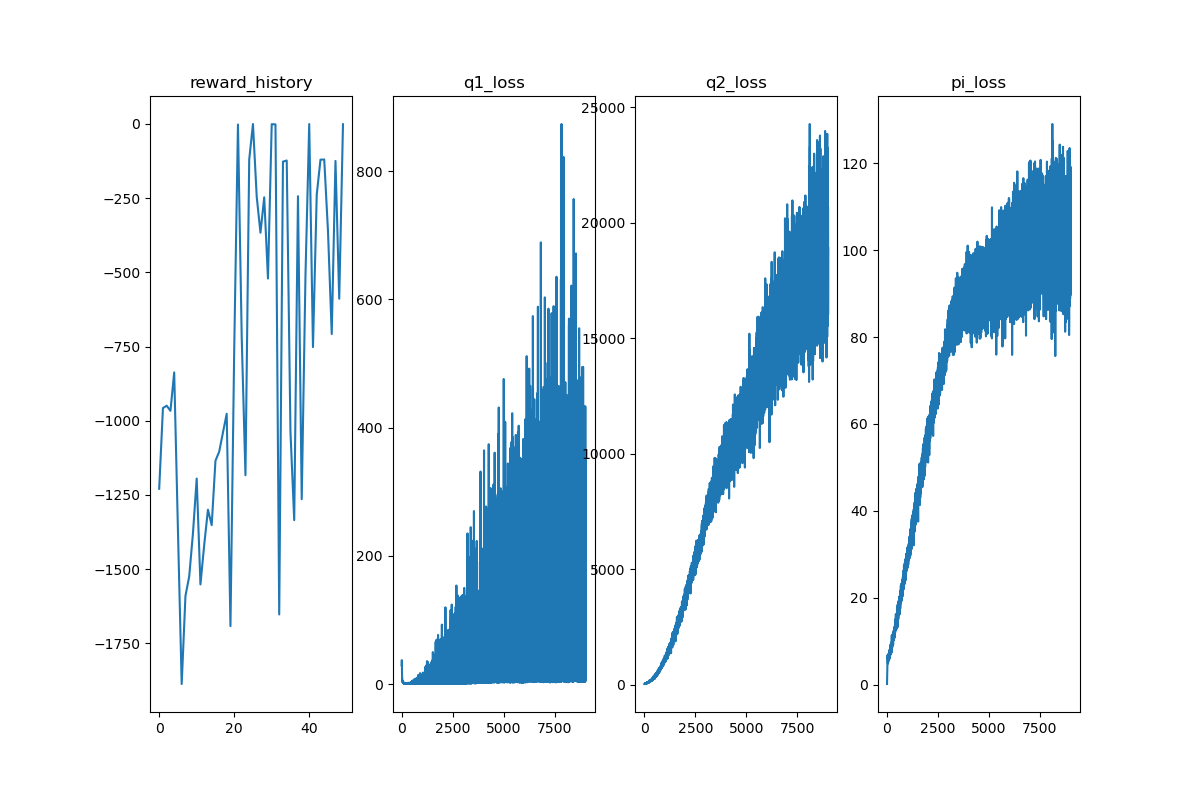
\includegraphics[width=0.45\textwidth]{sac-pendulum}
    \caption{SAC in the Pendulum-v1 Environment}
\end{figure}

\begin{figure}
    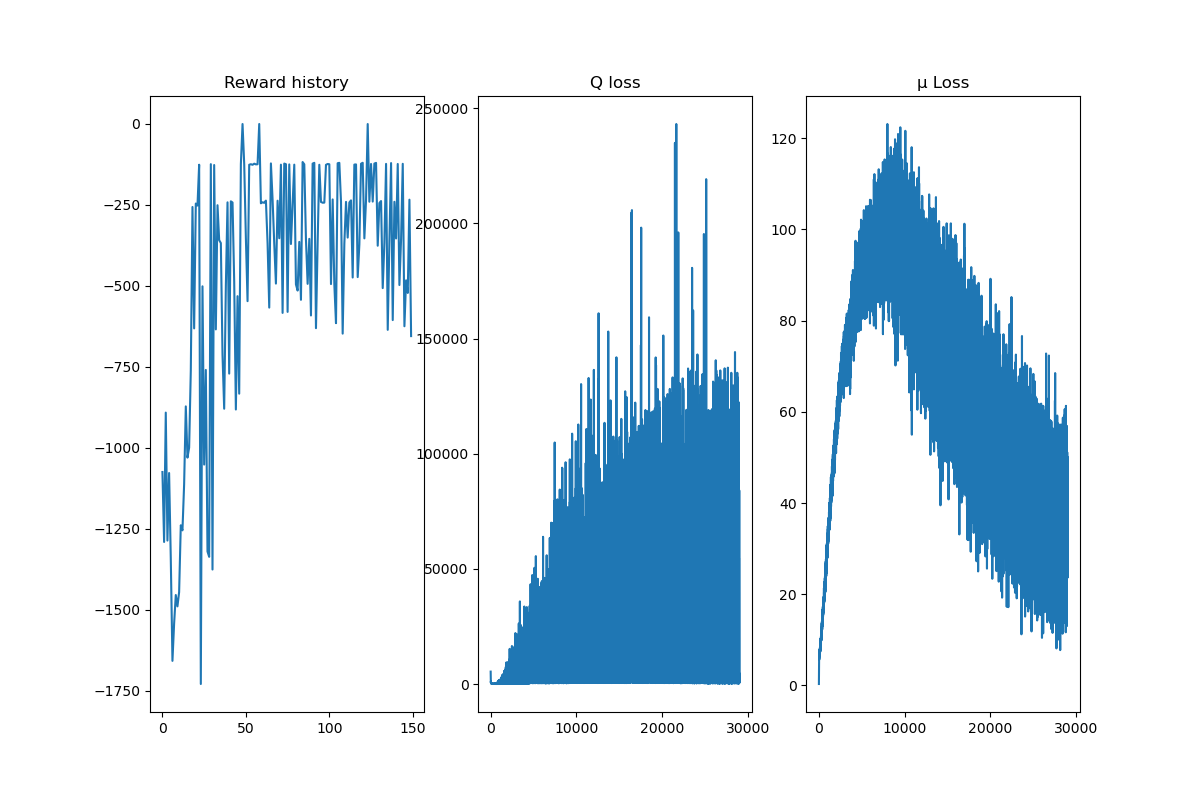
\includegraphics[width=0.45\textwidth]{ddpg-pendulum}
    \caption{DDPG in the Pendulum-v1 Environment}
\end{figure}

The tests on the pendulum environment proved that our implementations of A2C, DDPG and SAC were able to solve problems with continuous action spaces. Looking at the reward history in the Figures 1 and 2, it appears that DDPG was able to solve the algorithm faster than SAC. This isn't unexpected, considering that SAC uses significantly neural networks than DDPG and may take longer to train.

\subsection{Ant-v3}

\begin{figure}
    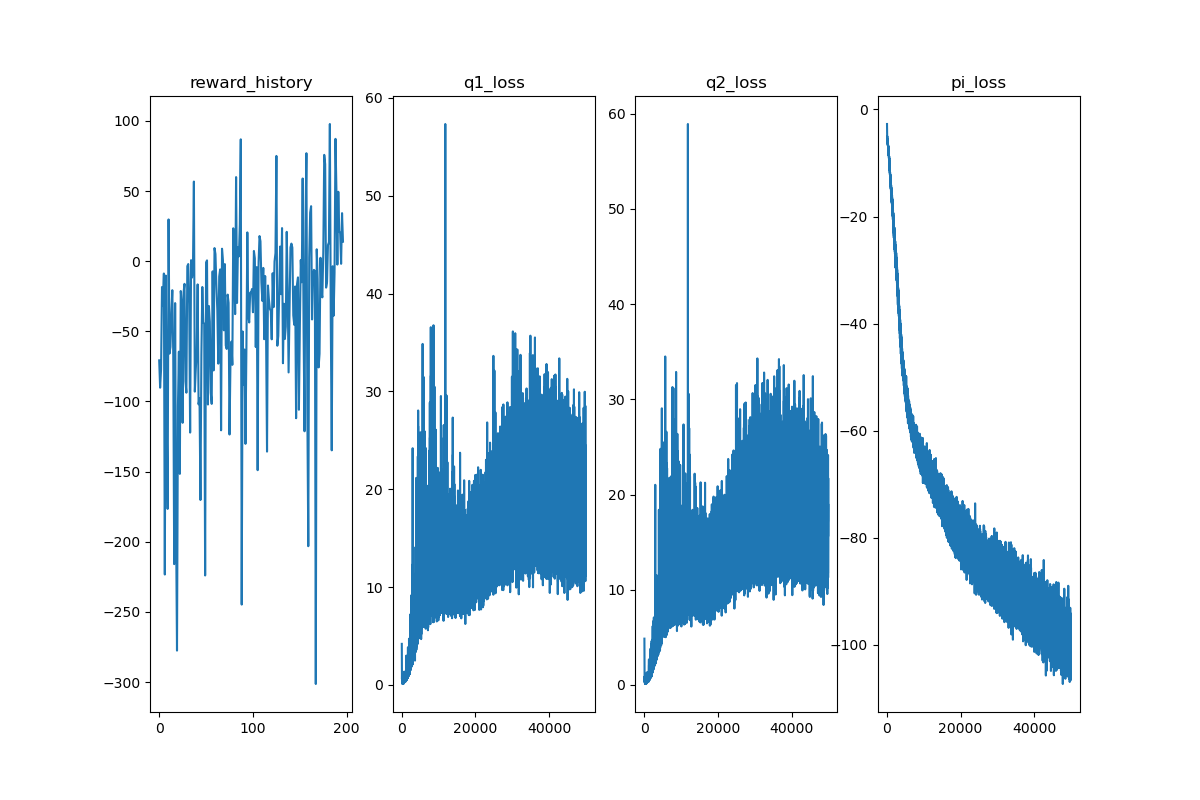
\includegraphics[width=0.45\textwidth, height=5cm]{sac-ant}
    \caption{SAC in the Ant-v3 environment}
\end{figure}

\begin{figure}
    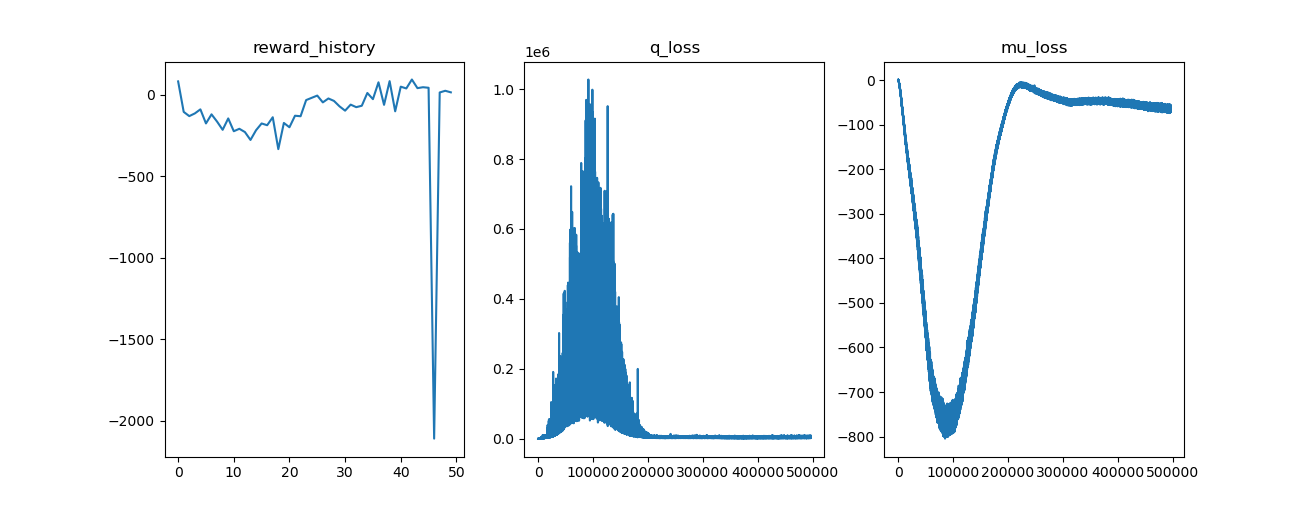
\includegraphics[width=0.45\textwidth, height=5cm]{ddpg-ant}
    \caption{DDPG in the Ant-v3 environment}
\end{figure}

\begin{figure}
    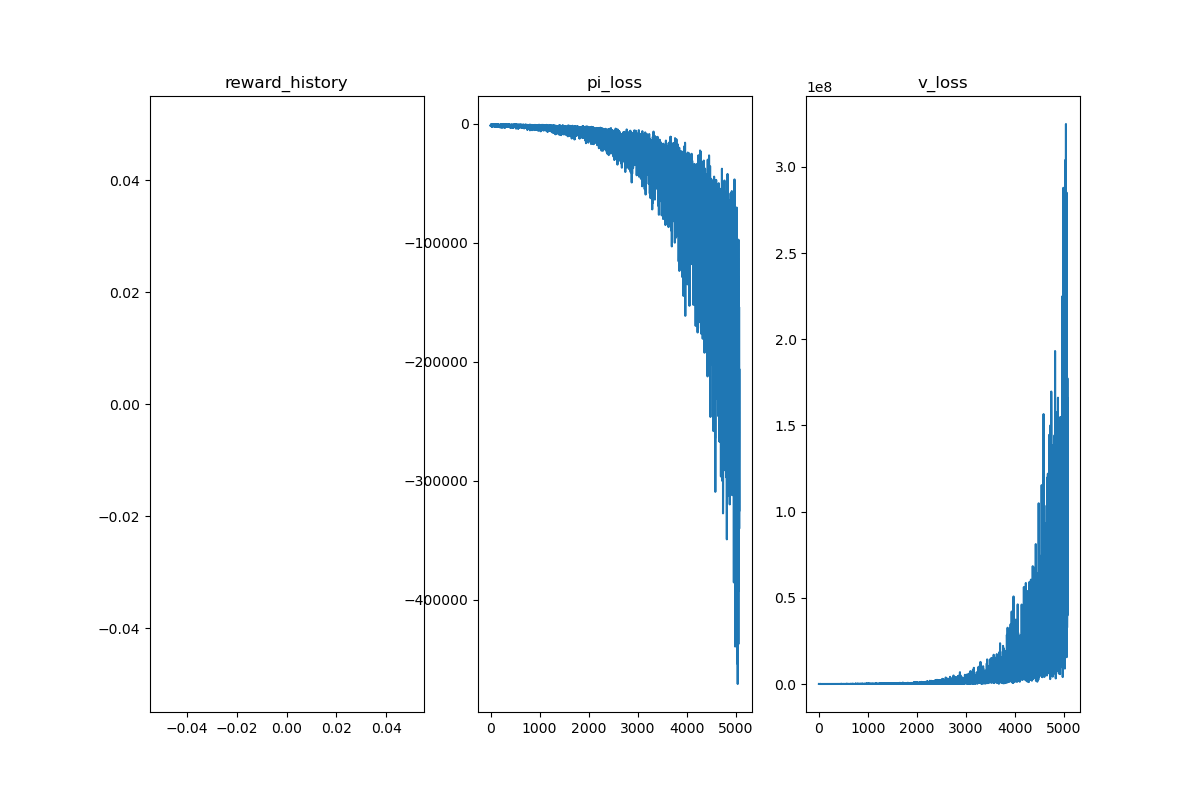
\includegraphics[width=0.45\textwidth, height=5cm]{a2c-ant}
    \caption{DDPG in the Ant-v3 environment}
\end{figure}



While each of the models were able to move the Ant model, they differed in the degree of "intelligence" they showed. Both A2C and DDPG learned to move the ant to the right, but their techniques were inconsistent and sporadic. Both methods frequently caused the ant to jump and flip around in the generally correct direction, but also frequently would get stuck upside down shortly after beginning.

DDPG was able to use the left and right legs to walk, and used the front and rear legs for steering. Using this method it was able to achieve quite the distance. But SAC managed to top even that; using the same locomotion scheme as DDPG, the model learned to leap through the air and even reached the edge of the floor in the environment. This is reflected in the performance graphs: the reward history for SAC increases at a steeper rate than it does for DDPG.

The main result from this test is that while all algorithms were able to make progress in the environment, SAC was able to significantly outperform the other algorithms. It learned to control the ant in a way that kept itself stable physically and move efficiently.

\subsection{Humanoid-v3}

\begin{figure}
    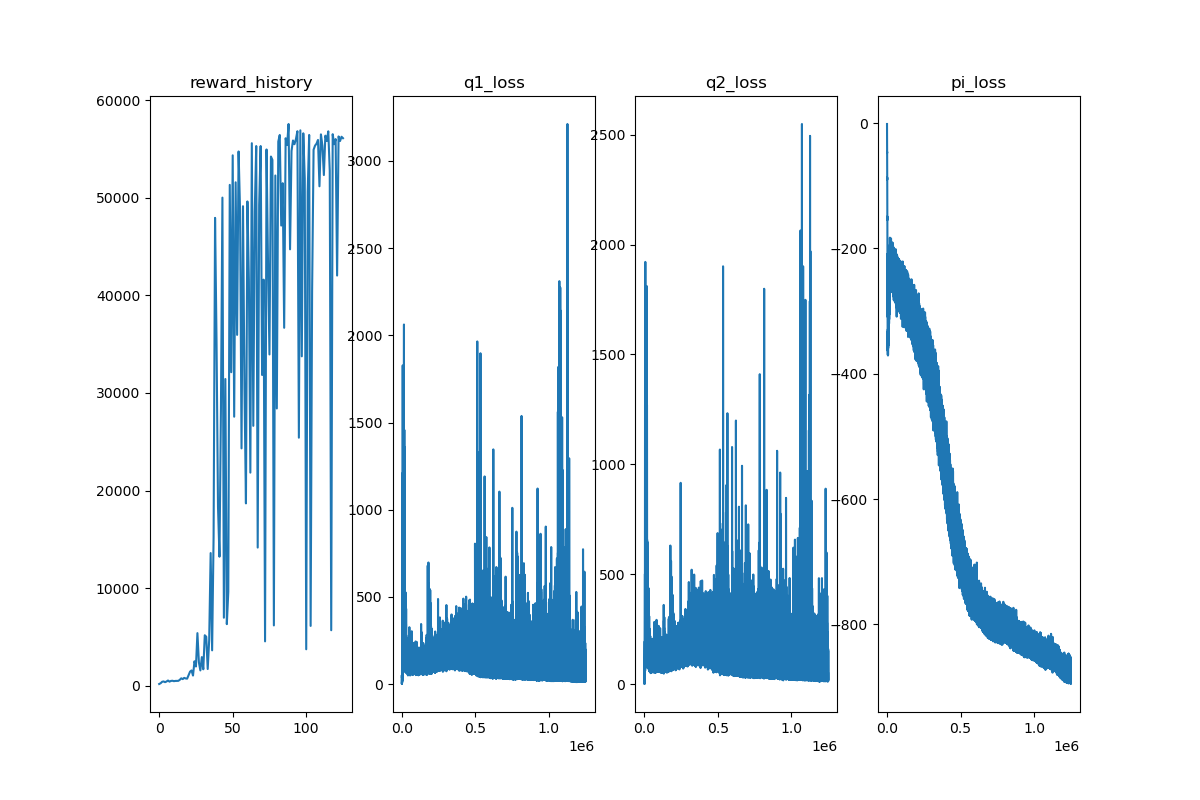
\includegraphics[width=0.45\textwidth, height=5cm]{sac-humanoid}
    \caption{SAC in the Humanoid-v3 environment}
\end{figure}

Since SAC's performance on the Ant model was so impressive, it was the first to train with the Humanoid model. As shown in the performance graph, it quickly learned how to walk using the arms for balance. After that initial hurdle, it refined its balance technique an opted for a slow and steady strategy by shuffling the feet along the floor. \textit {The SAC Shuffle} allowed the model to walk far into the distance, effectively solving the environment.

Unfortunately, the Humanoid-v3 environment was the most complex environment tested. The SAC model trained for 1,250,000 environment interactions which took over 12 hours using a NVIDIA RTX 3060 Ti. For this reason, testing algorithms we believed to be worse than SAC could not be justified due to time constraints.

\section{Conclusions and Future Work}

Learning to walk is a challenging problem; multiple limbs have to move in a coordinated fashion just to keep balance, adding movement on top of that is a problem that is potentially unsolvable with conventional programming methods. Using Reinforcement learning algorithms we were able to teach an agent to move a complex model in a 3D environment. Further, we found that some models such as SAC were able to learn complex behaviors such as leaping to improve its performance.

By implementing and training these algorithms, we are also leaping into success: we now have a solid foundation to begin building new experiences in Reinforcement Learning. We were introduced the foundations of RL like the value functions and policies, policy gradients, and a dictionary's worth of RL vocabulary. This knowledge of RL theory and application and is undoubtedly valuable for future projects in research and industry.

This project involving RL with MuJoCo could be continued in several different ways. One continuation we can explore would be implementing more algorithms or train with different kinds of environments that impose other interesting challenges. For example, can SAC learn to ride a bicycle? Another way to continue this project would be to explore the affects of hyperparameters in RL algorithms. Do certain hyperparameters affect training similarly between algorithms? How might they differ between algorithms? What are the optimal hyperparameters for different types of environments?

However, reinforcement learning has a much broader scope than just MuJoCo. The algorithms that we implemented could move on to Multiagent Learning for games like Chess \cite{multiagent}, learning how to play complex single player video games like Dark Souls, or even to control self driving vehicles \cite{self_driving}. Our new foundational knowledge of RL leaves us well equipped to keep up with research and contribute to the body of knowledge that is continuing to grow daily.

\bibliography{references}
\bibliographystyle{ieeetran}


\end{document}
